%!TEX root = ./sujet-projet.tex

\chapter{Analyse du domaine}\label{chapter:analyse}
\section{Introduction}

Dans ce chapitre, nous présentons l'ensemble des cas d'utilisation que nous avons dégagés lors de l'analyse du domaine. Nous utiliserons pour cela le canevas proposé par Cockburn~\cite{Cockburn:2000} que nous compléterons par des instantanés ainsi que par des post-conditions exprimées en OCL (Object Constraint Language) et quelques scenarii. Cette partie constitue une étape clé de la phase de spécification des besoins. 

Nous présentons également le diagramme des classes métiers (i.e., le diagramme de classes au niveau analyse) que nous avons construit à partir de l'analyse réalisée jusqu'à présent. 
Ce diagramme fournit une vue statique et synthétique du domaine ``\projet'' de notre application. 
Cette dernière partie constitue également une étape clé de la phase de spécification des besoins.


\section{Définition des cas d'utilisation}
Dans cette section, nous spécifions  l'ensemble des cas d'utilisation relatifs au domaine ``\projet''. Le diagramme présenté dans la Figure~\ref{fig:usecases} résume l'ensemble des cas d'utilisation associés de notre système. Ceux-ci peuvent être effectués par deux acteurs différents:
 \begin{itemize}
 \item Le chef de département;
 \item l'enseignant.
 \end{itemize}

\begin{figure}[h!]
	\centering
		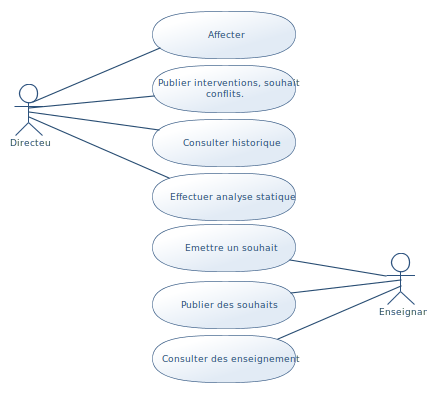
\includegraphics[scale=.7]{UC-Gestion Services.jpg}
	\caption{Cas d'utilisation du domaine "\projet".}
	 \label{fig:usecases}
\end{figure}

Dans les sections suivantes, nous fournissons une description plus détaillée de chacun des cas d'utilisation.

\subsection{UC---Affecter des enseignements}

\begin{usecase}{Affecter des enseignements}\label{usecase:affecter}
\begin{information}

 \item[Goal in the context:] Le chef de département réalise la confirmation d'un souhait d'un enseignant (validation) ou impose une intervention dans le département à un enseignant (affectation "forcée"). 
 L'enseignant devra se soumettre aux décisions du chef de département que ce soit pour une validation d'un souhait ou une affectation imposée.

\item[Scope:] Département

\item[{Level:}] Résumé (Summary)

 \item[{Precondition:}]
Le chef de département connait les souhaits (seulement ceux déjà publiés par l'enseignant), les possibles conflits et les affectations de l'enseignant concerné.

 \item[{Success End Condition:}]
L'enseignant est affecté à un ou plusieurs enseignements (souhait validé ou intervention imposée). 
Le volume horaire total effectué par l'enseignant a été recalculé.

 \item[{Failed End Condition:}]
 L'affectation n'a pas été réalisée (l'enseignement est déjà affecté à un autre enseignant : conflit).

\item[Primary actor:]
Chef de département.

 \item[Trigger:] Demande de réalisation d'une affectation faite par le chef de département.
\end{information}

\begin{scenario}
\item Le chef de département visualise l'ensemble des souhaits publiés par les enseignants.
\item Le chef de département sélectionne des souhaits, selon certains critères (l'enseignant, le module concerné, \dots).
%\item Le système renvoie les souhaits correspondants aux critères.  
\item Le chef de département choisit un vœu d'un enseignant afin de le valider.
\item Le chef de département valide le vœu, l'enseignement associé au vœu est affecté à l'enseignant concerné: c'est-à-dire que le vœu donne lieu à une intervention effective.
\item Le volume horaire des enseignants concernés est recalculé. 
\end{scenario}

 \begin{variation}
 \item [4] Le chef de département impose une intervention à un enseignant dans son département (affectation imposée).
 \item [4] Le chef de département valide une demande d'intervention extérieure ou une demande spéciale (remplacement, encadrement de stage, congés, \dots) de l'enseignant.
 % \item [4b1] Le système affecte l'intervention ou valide la demande spéciale de l'enseignant sans créer de conflits avec les autres enseignants.
 \end{variation}
\end{usecase}

\subsubsection{Spécification OCL}
\begin{ocl}
context UC::AffecterEnseignements(dep:Departement, voeux:Voeu[*])
post:
voeux->forAll(each:Voeux| let int = each.intervention in
	int.oclIsNew() and int.enseignant = each.enseignant and
	int.enseignement = each.enseignement)
	-- l`affectation d`un voeux crée une intervention dont l`enseignant et l`enseignement sont les mêmes que ceux du voeux.
 \end{ocl}

\begin{ocl}
context UC::AffecterDemandeExterieure(dep:Departement, d:DemandeExterieure)
post: let i = d.intervention in
	i.oclIsNew() and t.enseignement = d.enseignant and
	dep.interventions->includes(d.intervention)
-- l'affectaton d'une demande extérieure donne lieu à une intervention extérieure qui fait parti de 
-- la liste d'affectation de l'enseignant (celui qui a émis cette demande). 
-- Cette affectation est effectuée par le département.

\begin{ocl}
context UC::AffecterDemandeSpeciale(dep:Departement, ds:DemandeSpeciale)
post: let speciale = ds.intervention in
	speciale.oclIsNew() and speciale.enseignant = ds.enseignant
-- La DemandeSpeciale réalisée donne lieu à un CasSpecial qui fait parti de la liste d`affectation 
-- de l`enseignant (celui qui a émis cete DemandeSpeciale : de.emet). 
-- Cette réalisation est effectuée par le  département.
\end{ocl}

\begin{ocl}
context Departement::imposeInterventionDepartement(dep:Departement, ens:Enseignant, e:Enseignement)
post: Intervention.allInstances()->exists(i : Intervention |
	i.oclIsNew() and i.enseignement = e and i.enseignant = e)
-- L`enseignement est lié à une unique InterventionDepartement qui appartient à la liste des affectations 
-- de l'enseignant ens. C'est le département qui impose cette Intervention.
\end{ocl}


\subsubsection{Exemple d'affectation de voeux}
La Figure~\ref{fig:affectation} présente un exemple d'affectation des 3 voeux d'Alice et Bob.
L'affectation donne lieux à la création de trois instances d'intervention.

\begin{figure}[!htbp]
\begin{center}
\includegraphics[scale=.6]{OD-affecter-voeux}
\caption{Diagramme d'objets: Affecter des vœux}\label{fig:affectation}
\end{center}
\end{figure}

\subsubsection{Exemple d'affectation à partir d'une demande extérieure}
La Figure~\ref{fig:affectation:ext} présente l'affectation d'un voeu d'enseignement d'un intervenant extérieur, faite par l'enseignant Charles.
L'affectation à partir d'une demande extérieure crée une nouvelle intervention extérieure associée à la demande extérieure et à l'enseignant demandeur.

\begin{figure}[!htbp]
\begin{center}
\includegraphics[scale=.6]{OD-affecter-exterieur}
\caption{Diagramme d'objets: Affectation à partir d'une demande extérieure}
\label{fig:affectation:ext}
\end{center}
\end{figure}


\subsubsection{Exemple d'affectation à partir d'une demande spéciale}
La Figure~\ref{fig:affectation:spe} présente une affectation d'une demande spéciale de congé faite par l'enseignant Eve.
L'affectation une instance de  \code{CasSpécial} associé à l'enseignant et à la demande spéciale concernés.

 \begin{figure}[!htbp]
 \begin{center}
 \includegraphics[scale=.6]{OD-affecter-speciale}
 \caption{Diagramme d'objets: Affectation à partir d'une demande spéciale}
 \label{fig:affectation:spe}
 \end{center}
 \end{figure}

\subsubsection{Exemple d'affectation imposée à un enseignant}
La Figure~\ref{fig:affectation:imposee} présente une affectation imposée d'un enseignement de TP à l'enseignant Alice.
L'imposition d'une intervention à un enseignant crée une instance de la classe \code{InterventionDepartement} associée à l'enseignant et à l'enseignement concernés. Les interventions (dans le département) imposées ne sont pas liées à un vœu.

\begin{figure}[!htbp]
\begin{center}
\includegraphics[scale=.6]{OD-affecter-forcee}
\caption{Diagramme d'objets: Imposition d'une intervention à un enseignant}
\label{fig:affectation:imposee}
\end{center}
\end{figure}


\begin{comment}
	

 \subsubsection{Instantané: imposition d'une intervention à un enseignant par le chef de département}
 \begin{figure}[!htbp]
 \begin{center}
 \includegraphics[width=15cm]{fig/scenario3.jpg}
 \caption{Scénario : imposition d'une intervention à un enseignant par le chef de département}
 \end{center}
 \end{figure}

 Dans ce scénario, le chef de département impose une intervention concernant un enseignement de son département. L'affectation est donc imposée à l'enseignant.  

 \subsubsection{Instantané: imposer une affectation de type ``cas spécial'' (ex : arrêt maladie)}
 \indent Cas d'utilisation : \textbf{Réaliser une affectation} - Acteur : \textbf{Chef de département}

 \begin{figure}[!htbp]
 \begin{center}
 \includegraphics[width=14cm]{fig/10-ImpositionCasSpecial.jpg}
 \caption{Imposer une affectation de type ``cas spécial'' (ex : arrêt maladie)}
 \end{center}
 \end{figure}

 \indent L'imposition d'une affectation de type ``cas spécial'' à un enseignant crée une instance de la classe \textbf{CasSpécial} associée à l'enseignant concerné. Ce ``cas spécial'' n'est pas lié à une demande spéciale (puisqu'elle a été imposée).

 \begin{ocl}
 context Departement::imposeCasSpecial(ens : Enseignant, c : CasSpecial)
 post : ens.est_affecte_pour -> include(c)
 \end{ocl}
 \emph{Le CasSpecial c, appartient à la liste des affectations de l'enseignant ens. C'est le chef de département qui impose ce CasSpecial.}


%Afin d'avoir une vue plus globale de l'application, nous avons rédigé quelques scénarii faisant intervenir différents acteurs et différents cas d'utilisation. Ces scénarii sont exprimés sous la forme de diagrammes de séquence.

 \subsubsection{Conflit entre deux enseignants - résolution par le chef de département}
 \begin{figure}[!htbp]
 \begin{center}
 \includegraphics[width=15cm]{fig/scenario1.jpg}
 \caption{Scénario : conflit entre deux enseignants - résolution par le chef de département}
 \end{center}
 \end{figure}

Dans ce scénario, le conflit est réglé par le chef de département qui affecte l'enseignement à un seul des deux enseignants (la demande de l'autre enseignant est alors considérée comme étant refusée).

 \subsubsection{Conflit entre deux enseignants - résolution par un des enseignants}
 \begin{figure}[!htbp]
 \begin{center}
 \includegraphics[width=15cm]{fig/scenario2.jpg}
 \caption{Scénario : conflit entre deux enseignants - résolution par un des enseignants}
 \end{center}
 \end{figure}

 Dans ce scénario, le conflit est réglé par un des deux enseignants qui annule son vœu concernant l'enseignement à l'origine du conflit.  

\end{comment}

\subsection{UC---Valider des souhaits et publication des possibles conflits}

\begin{usecase}{Valider des souhaits et publication des possibles conflits}
\label{usecase:publier}
\begin{information}
	
\item[{Goal in the context:}]
 Le chef de département, par cette action, permet aux autres acteurs du système (en l'occurence les enseignants) de visualiser les informations concernant l'état actuel des souhaits de l'ensemble des enseignants. 
L'exécution de ce cas d'utilisation peut faire apparaître de nouveaux conflits pour les enseignants.

\item[Scope:] Département

 \item[{Level:}] Résumé

 \item[Precondition:] aucune

 \item[{Success End Condition:}]
Les enseignants ont accès aux informations concernant l'état actuel des souhaits publiés. 
Des conflits peuvent apparaître localement pour chaque enseignant.

 \item[{Failed End Condition:}]
 Echec de la publication : les enseignants n'ont toujours pas accès aux informations que le chef de département a tenté de publier.

\item[Primary actor:] Chef de département.

 \item[{Trigger:}]
 Demande de publication des interventions, des souhaits et des conflits possibles faite par le chef de département.
\end{information}

\begin{scenario}
\item Le chef de département visualise l'ensemble des souhaits non publiés.
% \item L'application renvoie l'ensemble des information voulues.
 \item Le chef de département sélectionne un ensemble de souhait et les valide.
 \item Le chef de département rend publics les souhaits validés.
 \item Le chef de département publie les nouveaux conflits qui sont apparus après la validation.
\end{scenario}

\end{usecase}

 \subsection{UC---Analyser des demandes}

\begin{usecase}{Analyser des demandes}\label{usecase:analyse}

\begin{information}
	

\item[Goal in the context:] Le chef de département effectue une analyse statistique permettant de déterminer la répartition des volumes horaires par enseignants ou la répartition des souhaits et affectations entre enseignants pour une année donnée. 

\item[Scope:] Département

\item[{Level:}] Résumé

\item[{Precondition:}]
 /

 \item[Success End Condition:]
/
% L'utilisateur visualise le résultat de l'étude statistique.

 \item[Failed End Condition:]
 /

 \item[Primary actor:]
 Chef de département.

 \item[Trigger:]
 Demande de réalisation d'un analyse statistique faite par le chef de département.\\
\end{information}

\begin{scenario}
	\item Le chef de département visualise les affectations (interventions) et les souhaits par rapport à une année donnée, selon un critère donné: par module, par enseignant, ou par le nombre d'heures effectives ou souhaitées.
	%\item Le chef département sélectionne les données qu'il désire ``analyser''. (cas d'utilisation n°3)
	\item Le chef de département analyse et corrige les affectations d'enseignement.
\end{scenario}

\end{usecase}

\subsection{UC---Émettre un souhait}

\begin{usecase}{\'Emettre un souhait}\label{usecase:souhait}
\begin{information}

\item [{Goal in the context:}]
 L'enseignant émet un souhait. Le souhait correspond à vœu sur un ensemble d'enseignements (avec une préférence) du département, une demande d'intervention extérieure au département ou une demande spéciale (arrêt maladie, remplacement,\dots)

\item[Scope:] Département

\item [{Level:}] Summary (Résumé)

\item[{Precondition:}]
 En cas de vœux sur des enseignements, ces derniers doivent exister et être non affectés à un autre enseignant.

\item[{Success End Condition:}]
 Le souhait de l'enseignant a été pris en compte mais n'est pas encore publié c'est-à-dire que seul l'enseignant peut le voir (i.e. cette modification est locale). 
Le volume horaire total (le volume horaire effectif plus la somme des volumes horaires des souhaits pas encore validés) de l'enseignant est modifié (recalculé) par rapport au volume horaire précisé dans le souhait.

\item[{Failed End Condition:}] L'enseignent n'arrive pas à émettre son souhait.
\item[{Primary actor:}] Enseignant.
\item[{Trigger:}] Demande d'émission d'un souhait faite par l'enseignant.
\end{information}

 %\noindent\textbf{MAIN SUCCESS SCENARIO}
 \begin{scenario}
	 \item L'enseignant recopie son souhait de l'année précédente.
	 \item L'enseignant visualise l'ensemble des enseignements disponibles (i.e. non affectés) dans son département.
	 \item L'enseignant fait son choix en sélectionnant un ensemble d'enseignements et indique son niveau de préférence pour ces enseignements (voulus ou seulement souhaités).
 \end{scenario}


\begin{extension}
 \item [3a.] Le vœu génère un conflit (avec d'autres souhaits déjà rendus publics) : le système le notifie à l'enseignant.
 \item [3b.] Le souhait génère un surplus d'heures pour l'enseignant (par rapport à son contrat de services) : le système le notifie à l'enseignant.
\end{extension}


\begin{variation}
	\item [1.] L'enseignant ne possède pas de historique de souhaits. Il commence avec un ensemble vide de souhaits.
	\item [3.] L'enseignant fait une demande concernant une intervention extérieure au département, précise le volume horaires et l'organisme concerné.
	\item [3.] L'enseignant décide de faire une demande spéciale souhaité en précisant le type (un congé, un remplacement, \dots) et le volume horaire.
\end{variation}
\end{usecase}

\subsubsection{Spécification OCL}
\begin{ocl}
context UC::EmettreVoeu(ens:Enseignant, m:Module, e:Enseignement, h: Integer, p:Integer)
post: 
ens.voeux->exists(v:Voeu| v.enseignement = e and v.volume = h and v.priorite = p)

-- Un nouveau voeu est ajouté à la liste des voeux de l`enseignant
\end{ocl}

\begin{ocl}
context UC::EmettreDemandeExterieure(ens:Enseigant, org:String, vol:Integer)
post: 
	ens.demandes->select(each | each.oclIsTypeOf(DemandeInterventionExterieure))->
		exists(d | d.oclIsNew() and d.volume = vol and d.organisation = org)
		
-- Une nouvelle demande d`intervention à l`extérieur est ajoutée à la liste de demandes de l`enseignant.
\end{ocl}

\begin{ocl}
context UC::EmettreDemandeSpeciale(ens:Enseignant, t:String, vol:Integer)
post:
	ens.demandes->select(each | each.oclIsTypeOf(DemandeSpeciale))->
		exists( d | d.oclIsNew() and d.volume = vol and d.type = t)

-- Une nouvelle demande spéciale est ajouté à la liste de demandes de l`enseignant.
\end{ocl}


\subsubsection{Exemple d'émission d'un souhait}
Dans cet exemple, l'enseignant Alice émet le souhait de réalise deux enseignements:
\begin{enumerate}
	\item Enseignement de 16h de CM du module Génie Logiciel;
	\item Enseignement de 16h de TD du module Réseaux.
\end{enumerate}
Le diagramme d'objets présenté dans la Figure~\ref{fig:souhait-alice} illustre ce souhait.
Après l'émission du souhait, une instance de la classe \code{Voeu} est créée pour chaque vœu, ainsi que deux liens, avec l'enseignant et l'enseignement concernés. 

 \begin{figure}[!htbp]
 \begin{center}
 \includegraphics[scale=.6]{"OD-alice-demande-gl"}
 \caption{Diagramme d'objets: Alice émet son souhait de service}
 \end{center}
 \label{fig:souhait-alice}
 \end{figure}


 \subsubsection{Exemple d'émission d'une demande extérieure}
Dans cet exemple, l'enseignant Bob fait une demande d'intervention de 12h à l'Institut Mines-Télécom Atlantique.
Le diagramme d'objets présenté dans la Figure~\ref{fig:demande:exterieure} illustre cette demande.
L'émission d'une demande extérieure crée une nouvelle demande extérieure associée à l'enseignant.
 
 \begin{figure}[!htbp]
 \begin{center}
 \includegraphics[scale=.6]{OD-emettre-demande-exterieure}
 \caption{\'Emission d'une demande d'intervention extérieure}
 \label{fig:demande:exterieure}
 \end{center}
 \end{figure}

 \subsubsection{Exemple d'émission d'une demande spéciale}
Dans cet exemple, l'enseignant Charles fait une demande de congés paternité, qui équivaut à 12h de décharge de service.
L'émission d'une demande spéciale crée la demande spéciale associée à l'enseignant.
\begin{figure}[!htbp]
\begin{center}
\includegraphics[scale=.6]{OD-emettre-demande-speciale}
\caption{\'Emission d'une demande spéciale}
\end{center}
\end{figure}




\subsection{UC---Publier des souhaits}
\begin{usecase}{Publier des souhaits}
\label{usecase:publier}
\begin{information}
	\item[Goal in the context:] L'enseignant transmet ses souhaits (préalablement sélectionnés) au chef de département qui sera lui même apte, dans un deuxième temps, à les rendre visibles à l'ensemble des enseignants.
Un souhait concerne un vœux fait sur des enseignements disponibles (i.e. non affectés), une intervention extérieure au département ou bien encore une demande caractérisée comme étant spéciale (congé, remplacement, \dots). 
	\item[Scope:] Département
	\item[Level:] Résumé
	\item[Precondition:] Le ou les vœux concernés ont été préalablement réalisés et validés localement par l'enseignant.
	\item[Success End Condition:] Le chef de département est capable de visualiser le/les souhaits publiés par l'enseignant.
	\item[Failed End Condition:] Le département ne reçoit pas les souhaits de l'enseignant.
	\item[Primary actor:] Enseignant.
	\item[Trigger:] Demande de publication de souhaits faite par l'enseignant.
\end{information}
\end{usecase}


\begin{scenario}
	\item L'enseignant choisit de visualiser l'ensemble des souhaits qu'il a réalisé localement mais qu'il n'a pas encore publié.
%	\item Le système lui renvoie l'ensemble de ces souhaits classés selon leur type (i.e. vœu, intervention extérieure et demande spéciale)
	\item L'utilisateur choisit, parmi ces souhaits, ceux qu'il désire publier et les transmet au chef de département.
	\item Le chef du département reçoit les vœux de l'enseignant.
\end{scenario}

 \begin{extension}
	 \item [2a.] Le système lui signifie qu'il n'existe pas de souhaits qui sont en attente d'être publiés.
	 \item [3a.] L'enseignant décide de ne publier aucun de ces souhaits et annule sa demande de publication.
	 \item [4a]. Le système signifie à l'utilisateur que l'un de ces souhaits (en l'occurence un vœu) concerne un ou plusieurs enseignements qui ont été affectés ou supprimés et lui demande de modifier son vœu.\\
 \end{extension}


 \subsection{UC---Consulter des enseignements}

\begin{usecase}{Consulter des enseignements}
\label{usecase:consulter}
\begin{information}
	\item[Goal in the context:]  L'enseignant doit être capable de visualiser les enseignements afin de consulter ou de modifier ses souhaits.
 Ainsi, des critères de tri sont mis à sa disposition pour personnaliser sa vue des enseignements dans le système "\projet": par module, par enseignement d'un module, par enseignant, ou par nombre d'heures.\\
 De plus, il doit choisir les critères de sélection des enseignements qu'il souhaite visualiser:
Les enseignements concernés par des vœux publiés ou non; les enseignements concernés par des vœux déjà validés (affectations);
ou les enseignements affectés et ceux non affectés.\\
 L'enseignant peut choisir de visualiser les enseignements des années précédentes mais il ne pourra effectuer aucune modification sur ces années. Par défaut, la visualisation se fera sur l'année en cours.
 L'utilisateur choisit l'ensemble des critères de tri et de sélection sur les enseignements qu'il souhaite. Il peut donc entièrement paramétrer sa vue des enseignements.
	\item[Scope:] Département
	\item[Level:] Résumé
	\item[Precondition:]/
	\item[Success End Condition:]/
	\item[Failed End Condition:]/
	\item[Primary actor:] Enseignant.
	\item[Trigger:] Demande de consultation des enseignements selon différents critères faite par l'enseignant.
\end{information}

\begin{scenario}
	\item L'enseignant décide de visualiser l'ensemble des enseignements selon ses critères.
	\item Le système renvoie l'ensemble des enseignements correspondants aux critères demandés.
\end{scenario}

 \begin{extension}
 \item [2a.] Le système ne renvoie rien puisqu'aucun enseignement ne correspond aux critères demandés.
 \end{extension}
\end{usecase}


\begin{comment}
 %*********
 \subsection{Instantanés et contraintes OCL sur les cas d'utilisation}
 \indent Nous allons vous présenter, dans cette sous-partie, un ensemble représentatif d'instantanés des cas d'utilisation. Nous allons donc partir d'un système vide (seul le département est représenté avec un module et deux enseignements) pour ensuite illustrer l'évolution de notre système au cours de son utilisation.\\
 \indent Voici le diagramme d'instances qui va nous servir de point de départ pour nos instantanés (nous considérons comme triviale la création des modules et des enseignements associés à un département) :

 \begin{figure}[!htbp]
 \begin{center}
 \includegraphics[width=4cm]{fig/base.jpg}
 \caption{Instantané de départ}
 \end{center}
 \end{figure}

 \subsubsection{Assigner un enseignant à un département}
 \indent Cas d'utilisation : non mentionné car basique - Acteur : \textbf{Chef de département}.

 \begin{figure}[!htbp]
 \begin{center}
 \includegraphics[width=12cm]{fig/1-assignEnseignant.jpg}
 \caption{Assignation d'un enseignant}
 \end{center}
 \end{figure}

 \indent L'assignation d'un nouvel enseignant au département provoque l'ajout d'une instance de la classe \textbf{Enseignant} ainsi que du contrat de service qui lui est associé (instance de la classe \textbf{ContratDeService}).

 \begin{verbatim}
 context Departement::assignerEnseignant(e : Enseignant)
 post : self.enseignant.include(e)
        and not e.contratdeservice.isUndefined()
 \end{verbatim}
 \emph{L'enseignant appartient au département et possède un contrat de service unique. L'assignation provient du chef de département.}







 \subsubsection{Assigner un responsable à un module}
 \indent Cas d'utilisation : \textbf{Assigner un responsable} - Acteur : \textbf{Chef de département}.

 \begin{figure}[!htbp]
 \begin{center}
 \includegraphics[width=12cm]{fig/4-ResponsableModule.jpg}
 \caption{Assignation d'un responsable à un module}
 \end{center}
 \end{figure}

 \indent L'assignation d'un responsable de module associe un enseignant au module dont il devient le responsable.

 \begin{verbatim}
 context Departement::assignerResponsable(m : Module, ens : Enseignant)
 post : m.est_responsable_de = ens
 \end{verbatim}
 \emph{L'enseignant ens devient responsable du module m. Cette assignation est réalisée par le chef de département}
\end{comment}

 \section{Diagramme de classes métiers}
Afin d'achever cette phase de spécification des besoins, nous fournissons une modélisation statique et synthétique du domaine de notre application. La figure~\ref{cls-metier} représente ce domaine "Gestion des services": 

 \begin{figure}[!htb]
 \centering
 \includegraphics[width=\linewidth] {CD-Gestion Services.jpg}
 \caption{Diagramme de classes métiers du domaine ``Gestion des services''}
 \label{cls-metier}
 \end{figure}

Le domaine "Gestion des services" est composé d'un ensemble de départements identifiés par leur nom (ex: département ``Informatique'', département ``Mathématiques'', \dots). 
Chacun de ces départements est constitué de parcours et possède un certain nombre d'enseignants qui lui sont rattachés.
Un parcours a un nom (ex: "Licence informatique", "Master Alma", etc.).

 Un module est défini par un nom, une année d'étude (ex: 2$^{\textrm{\footnotesize{e}}}$ année) et un semestre (1$^{\textrm{\footnotesize{e}}}$ ou 2$^{\textrm{\footnotesize{e}}}$). Il se décompose en plusieurs enseignements avec pour chacun un volume horaire et un coefficient: il peut s'agir de cours magistraux (CM), de travaux dirigés (TD) ou de travaux pratiques (TP). 
Chaque module a pour responsable un enseignant qui se doit, en principe, d'assurer un certain nombre d'enseignements dans ce module (le plus souvent les cours magistraux).

 Les enseignants sont caractérisés par leur nom et leur statut et doivent chacun remplir un contrat de service par année, c'est-à-dire effectuer un certain nombre d'heures minimum d'enseignement par année (calculé à partir des coefficients des enseignements). Il est important de noter que le contrat de service est uniquement fonction du statut de l'enseignant et est indépendant du département auquel il est rattaché.

 Chaque enseignant peut émettre un certain nombre de souhaits afin d'indiquer la manière dont il désire remplir son contrat de service. Ces souhaits peuvent être des vœux (indications du ou des enseignements que l'enseignant souhaite dispenser ainsi que ses préférences les concernant), des demandes d'intervention extérieure (dans une entreprise, une autre école...) ou des demandes spéciales (congés, arrêts maladie, encadrements de stages ou de TER\dots).

 Il est ensuite du ressort du chef du département concerné de décider de valider ou non ces souhaits, i.e. d'affecter ou non à l'enseignant concerné les interventions correspondantes aux souhaits émis. Toutefois, pour régler certains conflits, le chef d'un département se réserve le droit d'imposer une affectation à un enseignant sans que cet enseignant en ait auparavant formulé le souhait.

 % Pour terminer, notons que l'attribut nommé "année", présent dans la classe "Département", permet d'assurer la persistance des données concernant les modules, les enseignants, les souhaits et les interventions des différents enseignants au fil des années. Ainsi, il sera possible de construire un historique des souhaits et des interventions dans notre système. Cela pourra s'avérer très utile afin de permettre au chef de département de tenir compte des demandes des années passées pour le guider dans ses choix d'affectation concernant l'année en cours. Nous ne nous étendons pas sur le sujet de la persistance puisque ce n'est pas l'objectif de la phase de spécification des besoins.


